\chapter{Suffix Bomen}\label{ch:suffix-bomen}
Een eerste datastructuur die het mogelijk maakt om snel strings in een groot aantal andere strings te zoeken zijn suffix bomen.
Meer precies eigenlijk een gegeneraliseerde suffix boom.
\\ \\
De reden om deze datastructuur als eerste te behandelen is dat hij vrij intuïtief is en de makkelijkste van alle mogelijke opties.
Bovendien kan een goede tijdscomplexiteit bereikt worden aangezien het zoeken in een suffix boom in $O(n)$ kan (met $n$ de lengte van de zoekstring, in ons geval is dit een peptide).
Het opbouwen kan ook lineair gebruik makende van het algoritme van Ukkonen~\cite{Ukkonen1995}, met heeft een complexiteit van $O(m)$, met $m$ de som van de lengtes van alle proteïnes in de databank.


\section{Wat zijn suffix bomen?}\label{sec:wat-zijn-suffix-bomen?}
Suffix bomen zijn een soort veralgemening van tries (prefix bomen).
Door er voor te zorgen dat het laatste teken uniek is zal elke suffix van de input string uniek zijn (elke suffix is dus nooit de prefix van een andere suffix).
Dit zorgt er voor dat elke suffix een eigen blad in de boom zal krijgen.
Dit is dan ook van waar de naam suffix boom komt.
Elk pad tot een blad in de boom zal exact 1 suffix voorstellen uit de inputstring waarmee de boom gebouwd is.
Als voorbeeld stelt figuur~\ref{fig:suffix_tree_example} de suffix boom voor van de string \texttt{acacgt\$}.
Merk op dat we \texttt{`\$`} als uniek eindteken gebruiken.

\begin{figure}[H]
    \center
    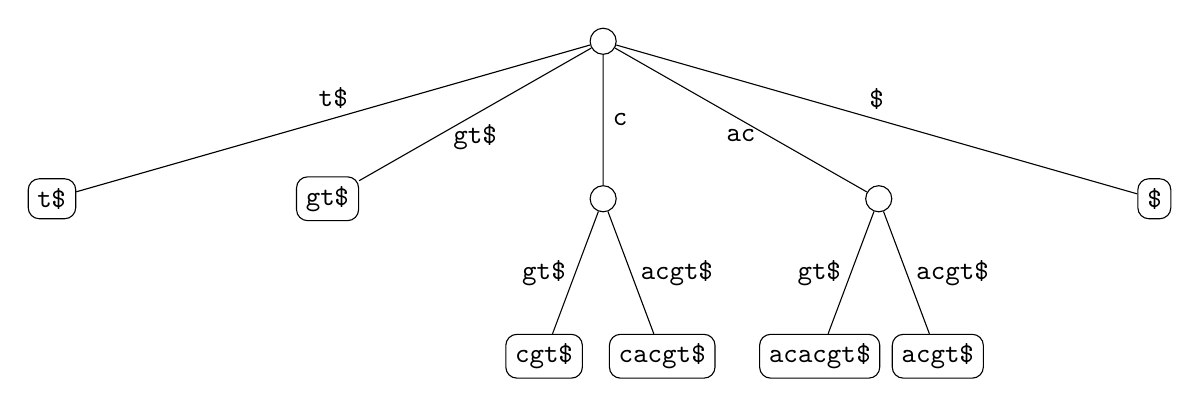
\begin{tikzpicture}
    [
        level 1/.style = {sibling distance = 3.5cm, level distance = 2cm},
        level 2/.style = {sibling distance = 1.5cm, level distance = 2cm}
    ]

        \node[draw, circle] {}
        child {
            node[draw, rounded corners] {\texttt{t\$}}
            edge from parent node [above] {\texttt{t\$}}
        }
        child {
            node[draw, rounded corners] {\texttt{gt\$}}
            edge from parent node [below] {\texttt{gt\$}}
        }
        child {
            node[draw, circle] {}
            child {
                node[draw, rounded corners] {\texttt{cgt\$}}
                edge from parent node [left] {\texttt{gt\$}}
            }
            child {
                node[draw, rounded corners] {\texttt{cacgt\$}}
                edge from parent node [right] {\texttt{acgt\$}}
            }
            edge from parent node [right] {\texttt{c}}
        }
        child {
            node[draw, circle] {}
            child {
                node[draw, rounded corners] {\texttt{acacgt\$}}
                edge from parent node [left] {\texttt{gt\$}}
            }
            child {
                node[draw, rounded corners] {\texttt{acgt\$}}
                edge from parent node [right] {\texttt{acgt\$}}
            }
            edge from parent node [below] {\texttt{ac}}
        }
        child {
            node[draw, rounded corners] {\texttt{\$}}
            edge from parent node [above] {\texttt{\$}}
        }
        ;
    \end{tikzpicture}
    \caption{Suffix boom voor the string \texttt{acacgt\$}}\label{fig:suffix_tree_example}

\end{figure}

Natuurlijk is dit niet efficiënt om effectief op deze manier op te slaan.
Als de tekst lengte $n$ heeft, heeft de suffix boom voor de tekst ten hoogste $2n - 1$ toppen en $2n - 2$ bogen.
Het aantal toppen en bogen is dus $\Theta(n)$.
Jammer genoeg vraagt alleen het opslaan van alle prefixen in de bladeren $\Theta(n^2)$ geheugen\cite{AD3_ukkonen}.
In de plaats kunnen we pointers bijhouden naar het begin en einde van een substring in de originele string.
Dit zorgt er voor dat we geen kopie meer moeten opslaan van de originele string in elk blad!
We moeten dit zelfs niet in elk blad bijhouden!
We kunnen simpelweg bij elke boog tussen de toppen de labels bijhouden.
Het label van het blad kunnen we daarna reconstrueren door de labels van de bogen op weg naar dit blad te concateneren.
Door dit te doen is de nodige opslag per top een constante, en is het geheugen gebruik lineair.
Figuur~\ref{fig:suffix_tree_example_indices} toont hoe dit er in de praktijk uit ziet.
Merk op dat de eind-index exclusief is.
Een boog met waarde \texttt{1,3}, stelt dus de substring \texttt{ca} voor uit het voorbeeld.

\begin{figure}[H]
    \center
    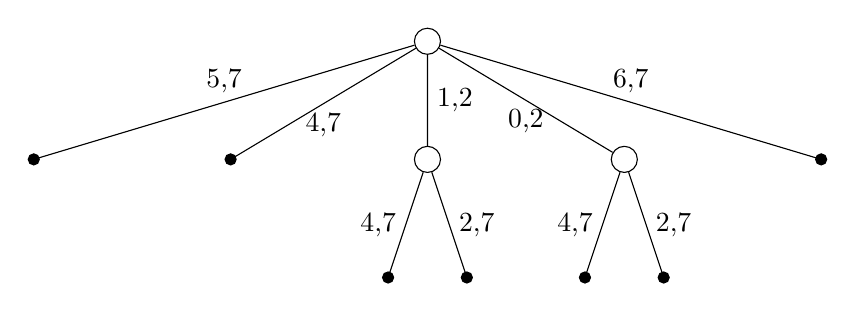
\begin{tikzpicture}
    [
        level 1/.style = {sibling distance = 2.5cm},
        level 2/.style = {sibling distance = 1cm}
    ]

        \node[draw, circle] {}
        child {
            [fill] circle (2pt)
            edge from parent node [above] {5,7}
        }
        child {
            [fill] circle (2pt)
            edge from parent node [below] {4,7}
        }
        child {
            node[draw, circle] {}
            child {
                [fill] circle (2pt)
                edge from parent node [left] {4,7}
            }
            child {
                [fill] circle (2pt)
                edge from parent node [right] {2,7}
            }
            edge from parent node [right] {1,2}
        }
        child {
            node[draw, circle] {}
            child {
                [fill] circle (2pt)
                edge from parent node [left] {4,7}
            }
            child {
                [fill] circle (2pt)
                edge from parent node [right] {2,7}
            }
            edge from parent node [below] {0,2}
        }
        child {
            [fill] circle (2pt)
            edge from parent node [above] {6,7}
        }
        ;
    \end{tikzpicture}
    \caption{Suffix boom voor de string \texttt{acacgt\$} gebruik makende van indices}\label{fig:suffix_tree_example_indices}

\end{figure}


\section{Ukkonen}\label{sec:Ukkonen}
Het algoritme van Ukkonen om suffix bomen op te bouwen staat gekend als vrij moeilijk.
Zeker de originele paper zelf is niet makkelijk verstaanbaar naar mijn mening en bevat weinig pseudocode.
Om dit beter te verstaan ben ik op zoek gegaan naar meerdere papers en boeken die dit algoritme in detail beschrijven.
Uiteindelijk kwam het grootste deel van de informatie van 3 verschillende plaatsen:
\begin{enumerate}
    \item Het boek \textit{Algorithms on Strings, Trees and Sequences}~\cite{Gusfield1997}.
    \item De cursus \textit{Algoritmen \& Datastucturen 3} aan UGent gegeven door prof. Gunnar Brinkmann~\cite{AD3_ukkonen}.
    \item De cursus Computational Challenges in Bioinformatics gegeven door prof. dr. Jan Fostier and prof. dr. Peter Dawyndt.
    Naast een cursus met wat info over het algoritme van Ukkonen is er ook een implementatie van dit algoritme gemaakt door Jan Fostier in C++ \footnote{\url{https://github.ugent.be/jfostier/CCB/tree/master/suffixtree}}.
\end{enumerate}

\subsection{Kotlin}\label{subsec:kotlin}
Om te beginnen heb ik eerst een implementatie van het algoritme van Ukkonen in Kotlin gemaakt zodat ik me niet op taal-specifieke problemen zou moeten focussen (vooral restricties rond borrowing in Rust).
Hier was gelukkig de referentie code van Jan Fostier een grote hulp omdat dit tijdens het mogelijk maakte om te zien wat de toestand van het programma zou moeten zijn na $x$ iteraties.
\\ \\
1 van de verschillen is dat ik hier toen gekozen heb voor een representatie van de kinderen aan de hand van een HashMap ipv een array van pointers, simpelweg uit gemak zodat ik rechtstreeks de characters als key kon gebruiken, en die niet moest omzetten naar een index.
De reden om Kotlin te kiezen en niet Python is simpelweg performantie aangezien het in kotlin nog doenbaar was om de test datasets op te bouwen in een redelijke tijd.
\\ \\
Uiteindelijk bleek de grootste struikelblok in het implementeren van het Ukkonen enkele off-by-1 errors.
Aangezien je tijdens het algoritme eigenlijk werkt met substrings, maar deze opgeslagen worden aan de hand van hun begin- en eind-index wordt het debuggen veel omslachtiger.
Tijdens het debuggen zie je namelijk enkel ``ik ben nu in top $y$ die de substring van index $i$ tot index $j$ voorstelt, en de kinderen stellen de substring $k$ tot $l$, \ldots voor''.
Tot slot had ik op het einde ook enkele bugs die niet voorkwamen in kleinere voorbeelden die nog met de hand uit te werken waren, wat daardoor relatief wat tijd vroeg om op te lossen.

\subsection{Rust}\label{subsec:rust}

\subsubsection{Eerste ervaring}
Aangezien dit mijn eerste ervaring was met Rust deel ik graag even mijn eerste bevindingen mee.
Zelf heb ik eerst \textit{the Rust book} gelezen~\cite{the_rust_book}.
Wat op zich veel goede informatie heeft, maar naar mijn ervaring soms te veel.
Een veelvoorkomend patroon in het boek is dat een deel van een concept geïntroduceerd wordt en dat je dan als lezer geïnformeerd wordt dat je er nu nog niet over moet denken, dat er meer informatie hierover komt in een later hoofdstuk.
Dit zorgt ervoor dat het soms moeilijk is de bomen door het bos te zien.
Zeker aangezien Rust vaak verschillende syntaxen heeft om hetzelfde te doen, waardoor je als lezer moeilijk je kunt focussen op de essentiële delen.
\\ \\
Om de meest essentiële basis componenten van Rust wat onder de knie te krijgen heb ik daarna de oefeningen van Rustlings~\cite{rustlings} gemaakt op aanraden van mede thesis student Stijn De Clercq.
Dit zijn een reeks aan erg kleine oefeningen die meestal in maximaal enkele minuten gemaakt zijn, maar er voor zorgen dat je toch al eens in contact komt met alle basisonderdelen van Rust.
Naar mijn mening is dit dus zeker een waardevolle toevoeging tijdens het leren van Rust.

\subsubsection{Boomstructuren}
\begin{quote}
    \textit{Rust is known to be notorious difficult when it comes to certain data structures like linked lists, trees, etc. \cite{rust_difficulty_quote}}
\end{quote}
Deze quote komt rechtstreeks uit een Medium artikel en toont direct dat het maken van een suffix boom in Rust niet-triviaal ging zijn.
De oorzaak hiervoor ligt bij het \textit{ownership} systeem van Rust.
Dit systeem zorgt er voor dat slechts 1 variabele eigenaar kan zijn van een stukje data.
In dit geval kan dus slechts 1 top een andere top opslaan, of er een \textit{mutable reference} naar hebben.
Meer praktisch wil dit dus zeggen dat slechts 1 top een pointer kan hebben naar een andere top, met de toelating om die top aan te passen (wat nodig is tijdens het opbouwen van de boom, waarin kinderen nog toegevoegd worden, toppen moeten gesplitst worden enz.)
Dit is een groot probleem aangezien ouders pointers naar kinderen moeten hebben, de kinderen een pointer naar hun ouder, en er dan ook nog eens pointers zijn voor de suffix links.
Dit gaat duidelijk niet zomaar voldoen aan het ownership systeem!
\\ \\
Als oplossing hiervoor introduceert Rust het \texttt{Rc<T>} datatype.
Hierbij gaat Rust afstappen van zijn standaard ownership systeem en gebruik maken van Reference Counting.
Pas wanneer alle references weg zijn zal het geheugen automatisch vrij gegeven worden.
De beperking hierbij is echter dat deze referenties \textit{immutable} zijn, dit voldoet niet tijdens het opbouwen van de boom.
\\ \\
Als oplossing hiervoor heeft Rust dan weer het \textit{interior mutability} patroon~\cite{interior_mutability} aan de hand van het datatype \texttt{Refcell}.
Dit laat toe om data toch aan te passen, ook al is een reference immutable.
Aangezien dit de standaard Rust regels doorbreekt, is dit \texttt{unsafe} en kan Rust \textit{at compile-time} geen \textit{memory safety} meer garanderen.
\texttt{Refcell} zal gelukkig wel de nodige code invoegen zodat runtime memory safety wel gegarandeerd kan worden.
Mogelijke foutieve geheugen operaties zullen dus tijdens het uitvoeren van het programma gedetecteerd worden, \textbf{ten koste van performantie}.
\\ \\
Maar zelfs nu blijft er nog altijd een probleem.
Geheugen aan de hand van reference counting zal enkel vrijgegeven kunnen worden indien de reference counter op 0 staat.
Er zijn echter scenario's waar dit nooit zal gebeuren.
Namelijk bij cyclische verwijzingen, een patroon dat jammer genoeg erg vaak voor komt (in ons geval bv een ouder die een pointer heeft naar een kind, en een kind een pointer naar de ouder).
Als oplossing hiervoor introduceert Rust dan weer het \texttt{Weak<T>} datatype.
\\ \\
Dit is duidelijk erg ingewikkeld, en introduceert ook nog eens performance overhead die niet nodig lijkt.
Een optie zou natuurlijk zijn door expliciet het \texttt{unsafe} keyword te gebruiken wat toe laat de ownership regels van Rust volledig uit te schakelen (zowel compile-time als run-time).
Het nadeel hiervan is natuurlijk dat we dan de garanties van memory safety kwijt zijn, wat net 1 van de hoofdredenen is om Rust te gebruiken.
Dit was dus geen mogelijke optie.
Gelukkig is er een alternatieve manier waar ik op gestoten ben, een arena-based implementatie~\cite{rust_arena_trees}.
Het idee hierbij is dat er 1 arena gemaakt wordt waarbij ownership erg simpel is.
In mijn implementatie is dit bijvoorbeeld een \texttt{Vector}.
Alle toppen worden hierbij in deze ene vector opgeslagen.
In plaats van pointers naar elkaar houden, zullen de toppen indexen bijhouden.
Deze index stelt de index in de arena van de top voor waarnaar anders een pointer wordt bijgehouden.
\\ \\
Na het maken van deze ontwerpaanpassingen bleef slechts 1 moeilijkheid over.
Uitzoeken hoe de cursor (die bij houdt waar we zijn in de boom tijdens het bouwen), de input string en de boom zelf zich van elkaar moeten verhouden in het ownership systeem.
Uiteindelijk viel dit vrij makkelijk uit te zoeken.
Het omzetten van de resterende Kotlin code naar Rust was erg simpel en bijna een één op één vertaling.
Het enige verschil is dat ik in de Rust implementatie gebruik heb gemaakt van een array om de kinderen bij te houden in plaats van een HashMap.

\subsubsection{Geheugen efficiëntie}
\begin{quote}
    \textit{And then I went and invented a null pointer.
    And if you use a null pointer you either have to check every reference or you risk disaster. \cite{null_mistake}}
\end{quote}
Null-pointers worden ook wel \textit{the billion-dollar mistake} genoemd vanwege het grote aantal bugs dat veroorzaakt worden door null pointers.
Daarom voorziet Rust een andere manier om de waarde ``null'' voor te stellen.
Dit wordt gedaan aan de hand van de \texttt{Option<T>} enum.

\begin{minted}{Rust}
enum Option<T> {
    None,
    Some(T),
}
\end{minted}

Deze enum heeft 2 mogelijke waarden: \texttt{None} of \texttt{Some(T)}.
\texttt{None} is het equivalent dat overeen komt met null, terwijl \texttt{Some(T)} wil zeggen dat de waarde niet-null is, en meer specifiek is de waarde \texttt{T}.
Aangezien het grootste deel van wat bijgehouden wordt per top eigenlijk pointers zijn maakte ik veelvoudig gebruik van deze Option-enum.
Alle pointers in een top kunnen namelijk null zijn!
De parent pointer moet nullable zijn aangezien de root geen parent heeft, de child pointers moeten allemaal nullable zijn omdat bladeren geen kinderen hebben (en in de interne toppen zijn niet alle kinderen altijd nodig) en de suffix-links moeten nullable zijn aangezien niet elke top een suffix link heeft naar een andere top.
\\ \\
Dit werkte perfect en kon proper afgehandeld worden op de idiomatische manier die overeenkomt met propere Rust code.
Na de eerste benchmarks bleek het geheugengebruik echter problematisch.
Bijna exact 2x zo hoog als de equivalente C++ implementatie.
Om zo'n drastisch verschil in geheugenverbruik te kunnen verklaren moest er wel iets fundamenteel verschillen aan de manier dat toppen hun data bijhouden.
Al snel bleek dat het gebruik van \texttt{Option<usize>} als datatype in plaats van \texttt{usize} 8 bytes aan overhead per index had!
Dit is inderdaad exact het dubbele geheugenverbruik op een 64-bit machine aangezien een \texttt{usize} 8 bytes groot is.
Dit valt makkelijk te controleren aan de hand van de \texttt{std::mem::size\_of} functie deel van de Rust standaard bibliotheek.
Onderstaand voorbeeld toont dat dit inderdaad het geval is.
\begin{minted}{Rust}
assert_eq!(mem::size_of::<Option<usize>>(), 16);
assert_eq!(mem::size_of::<usize>(), 8);
\end{minted}

Als oplossing heb ik uiteindelijk mijn eigen ``null'' value gedefinieerd gebruik makende van een Trait.
Deze oplossing verslaat volledig het doel van de \texttt{Option<T>} enum, maar is jammergenoeg nodig omdat het gewoonweg niet acceptabel is het geheugenverbruik te verdubbelen hiervoor.
Bovendien blijft memory safety gegarandeerd aangezien het foutief indexeren van de NULL-value (\texttt{usize::MAX} in dit geval) een index-out-of-bounds error creëert.
Wat tijdens runtime gedetecteerd wordt en dus geen verdere problemen geeft (buiten dat het programma zal crashen).

\begin{minted}{Rust}
/// Custom trait implemented by types that have a value that represents NULL
pub trait Nullable<T> {
    const NULL: T;

    fn is_null(&self) -> bool;
}

/// Type that represents the index of a node in the arena part of the tree
pub type NodeIndex = usize;

impl Nullable<NodeIndex> for NodeIndex {
    /// Use usize::MAX as NULL value since this will in practice never be reached.
    /// It is not possible to create 2^64-1 nodes (on a 64-bit machine).
    /// This would simply never fit in memory
    const NULL: NodeIndex = usize::MAX;

    fn is_null(&self) -> bool {
        *self == Self::NULL
    }
}
\end{minted}

\subsection{Performantie}\label{subsec:performantie}
Natuurlijk is het belangrijk dat de implementatie performant (en correct) is.
Aangezien er een bestaande C++ implementatie was van Ukkonen in C++ was dit een perfecte maatstaf.

Uiteindelijk heb ik 1 aanpassingen moeten maken in de C++ code die al bestond om een eerlijke vergelijking uit te voeren.
Oorspronkelijk werd er in elke top plaats gehouden voor 256 mogelijke kinderen.
Dit was veel te hoog voor deze usecase waardoor het geheugenverbruik dramatisch groot was (ongeveer een factor 10 hoger dan wat nodig was).
Uiteindelijk ben ik gegaan voor een implementatie (zowel in Rust als C++) waarin plaats gehouden wordt voor 28 kinderen.
Dit zijn de 26 letters van het alfabet + \texttt{`\#`} + \texttt{`\$`}.
De reden om \texttt{`\#`} en \texttt{`\$`} ook te gebruiken is omdat er een scheidingsteken nodig is tussen de sequenties (in deze implementatie \texttt{`\#`}) en een uniek teken op het einde (de \texttt{`\$`}).
Dit is ook wat al gebeurde in de bestaande C++ implementatie.

Een andere aanpak zou kunnen zijn om HashMaps te gebruiken.
Het totale geheugenverbruik zal hierdoor afnemen naar ongeveer 60\% van het huidige verbruik, maar ten koste van performantie tijdens het zoeken (wat net erg belangrijk is).
Hoe dan ook blijft het geheugen verbruik extreem groot, welke implementatie ook gekozen wordt.
\\ \\
Het vergelijken van de implementaties heb ik opgesplitst in 2 stukken:
\begin{enumerate}
    \item het opbouwen van de index-structuur.
    \item Zoeken in de index-structuur
\end{enumerate}

\subsubsection{Opbouwen}
Om een representatief resultaat te krijgen is het opbouwen van de boom 10x uitgevoerd en zijn de gemiddelden van de resultaten genomen.
Om de uitvoeringstijd en het geheugenverbruik te meten heb ik gebruik gemaakt van het \texttt{time} commando.
De resultaten hiervan zijn terug te vinden in figuur~\ref{fig:tree_building}.
\begin{figure}[H]
    \centering
    \subfloat[Tijd nodig om de boom op te bouwen]{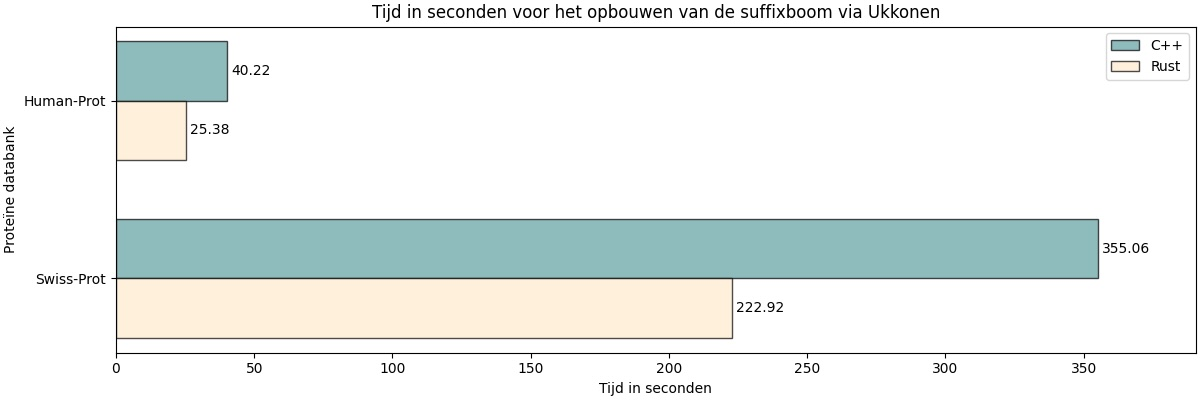
\includegraphics[width=\linewidth]{building_tree_time}}\\[4ex] % [4ex] om wat extra vertical spacing in te voegen

    \subfloat[Maximaal gebruikt geheugen tijdens het opbouwen van de boom]{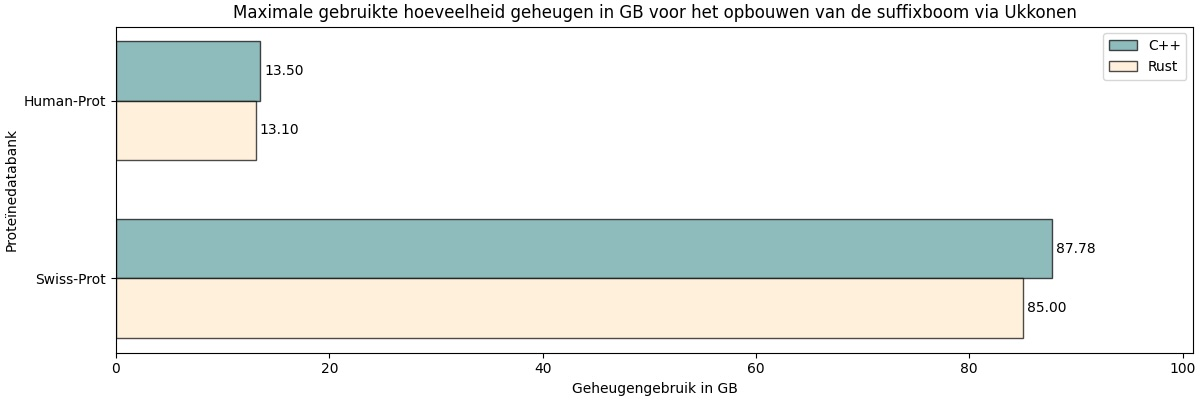
\includegraphics[width=\linewidth]{building_tree_memory}}
    \caption{Vergelijking van C++ en Rust voor het opbwouven van de suffix boom}\label{fig:tree_building}
\end{figure}

Uit deze grafieken vallen 2 duidelijke conclusies te trekken.
\begin{enumerate}
    \item De implementatie in Rust is $\pm$ 33\% sneller
    \item Het geheugenverbruik is erg vergelijkbaar.
    Dit valt te verwachten aangezien beide implementaties 8 bytes nodig hebben per \textit{pointer} en evenveel plaats voorzien voor de kinderen.
    Het kleine verschil valt te verklaren vanwege 1 veld dat ik niet bij houdt tijdens het opbouwen, dat wel gebruikt wordt in de C++ implementatie.
    Dit is de diepte van de top in de boom.
    Op de enkele plaatsen waar dit nodig is kan ik gebruik maken van andere variabelen om tot een equivalent resultaat te komen.
\end{enumerate}

\subsubsection{Zoeken}
Bij het zoeken zijn er 2 belangrijke manieren om te vergelijken.
\begin{enumerate}
    \item Zoek totdat we weten als er een match bestaat voor de peptide of niet, en stop dan.
    \item Zoek totdat er een match is, en doorzoek daarna de volledige sub-boom om alle informatie van de kinderen op te halen.

\end{enumerate}

\paragraph{Zoek een match}
De reden voor deze manier van zoeken is dat het mogelijk is om info te propageren van de bladeren tot bovenin de boom.
In ons geval is dit bijvoorbeeld de LCA van de taxon IDs op voorhand te berekenen.
Het zoeken van de LCA die overeenkomt met alle proteïnen waar de gevonden peptide mee matcht kan dus al stoppen vanaf er een match is.
\\ \\
Grafiek~\ref{fig:performance_match_tree} toont de nodige tijd om alle peptiden van de gebruikte zoekbestanden 1x te zoeken totdat er een (mis)match was voor de peptide.
De grafiek bevat de gemiddelde resultaten van 5000 \textit{runs}, maar zelfs dan bleven de resultaten wat schommelen.
Doordat de te meten tijd zo klein is, kan de kleinste invloed al voor een zichtbaar verschil zorgen.
Dit kan bv een achtergrond proces zijn, maar ook invloed van een andere VM die op de fysieke machine bezig is (wat hier het geval is, aangezien Stijn De Clercq ook een VM op \textit{Matty} gebruikt voor zijn testen).
Dit was ook merkbaar tijdens het testen waar dat de verschillen tussen 2 opeenvolgende uitvoeringen vaak groter waren dan het verschil tussen de C++ en Rust implementatie.
Toch kunnen we besluiten dat de C++ implementatie een beetje performanter zal zijn aangezien dit in elk zoekbestand (nipt) sneller is (soms zelfs minder dan een milliseconde!).

\begin{figure}[H]
    \centering
    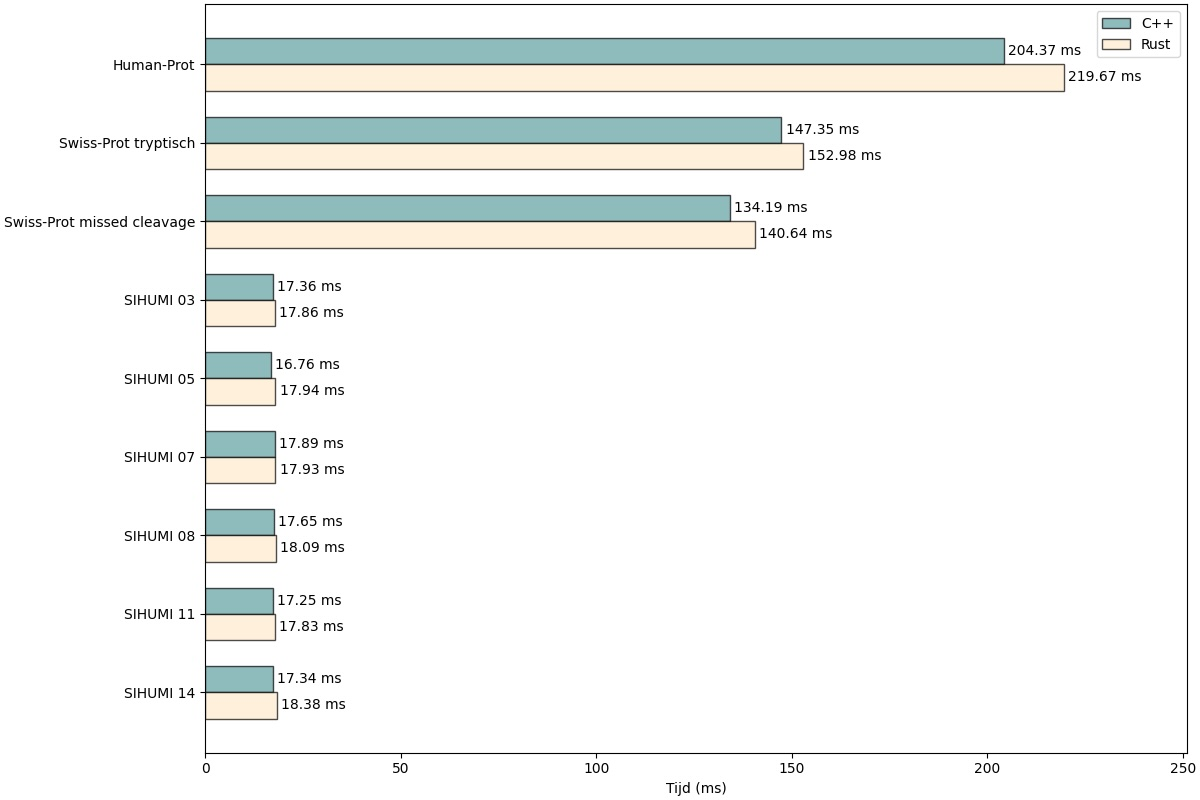
\includegraphics[width=\linewidth]{search_match_performance_tree}
    \caption{Uitvoeringstijd voor het zoeken tot een match voor alle zoekbestanden}
    \label{fig:performance_match_tree}
\end{figure}

Dit is verbijsterend snel vergeleken met de huidige implementatie in Unipept.
Daar duurt het op dit moment 2 minuten en 12 seconden om alle peptiden van het Swiss-Prot zoekbestand zonder \textit{missed cleavages} te zoeken,
en maar liefst 30 minuten 37 seconden voor het zoekbestand met \textit{missed cleavages}!
Dit is maar liefst $\frac{132 000}{152.98} = 857$ en $\frac{1 837 000}{140.64} = 13 000$ keer trager!
Als keerzijde van de medaille gebruikt Unipept op dit moment hiervoor slechts 6.7 GiB geheugen, en dit kan zelfs nog naar beneden.
Dit is ongeveer 13 keer lager!

\paragraph{Zoek match en haal informatie over kinderen op}
De reden dat dit belangrijk is, is dat alle bladeren in deze sub-boom de proteïnen voorstellen waar dat de gevonden peptide een deel van is.
De relevante informatie over de huidige peptide is daarom de informatie dat verbonden is aan deze proteïnen. % TODO: voor wat konden we dit ook nog gebruiken?

Figuur~\ref{fig:performance_all-occurrences_tree} bevat een overzicht van de nodige zoektijd voor beide implementaties op alle zoekbestanden.
We zien duidelijk dat er hier een gigantisch verschil is tussen de C++ en Rust implementatie.
Vermoedelijk komt dit door de andere memory layout die ontstaat doordat de Rust implementatie 1 grote Vector gebruikt, terwijl de C++ implementatie losse toppen gebruikt die verspreid liggen in het geheugen.

\begin{figure}[H]
    \centering
    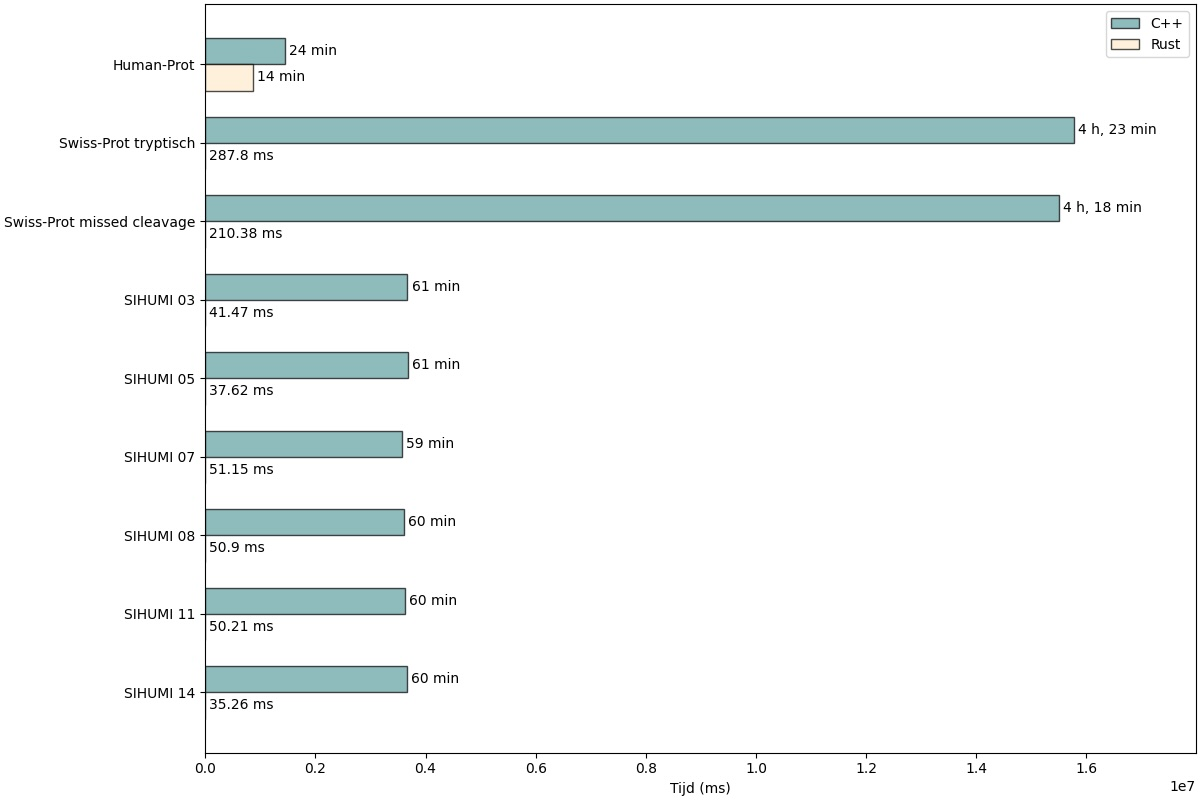
\includegraphics[width=\linewidth]{search_all-occurrences_performance_tree}
    \caption{Uitvoeringstijd voor inclusief het doorzoeken van de volledige subboom na match voor alle zoekbestanden}
    \label{fig:performance_all-occurrences_tree}
\end{figure}


\section{Taxon ID aggregatie}\label{sec:taxon-id-aggregatie}
Mogelijks het belangrijkste stukje info over een staal peptiden is weten van welke organismen dit komt.
Aangezien peptiden kunnen matchen met proteïnen die uit verschillende organismen komen moet er een manier gekozen worden om deze informatie te aggregeren, of te beslissen van welk organisme dit komt met de grootste kans.
Aangezien er geen manier is om met zekerheid te zeggen uit welke proteïne de peptide komt (als er meerdere opties zijn) gaat Unipept de info gaan veralgemenen.
Anders gezegd: Unipept zal enkel info geven die geldt op alle gematchte proteïnen.
1 van deze stukjes informatie is het Taxon ID\@.
Ipv een lijst van alle mogelijke ID's te geven (wat een extreem grote lijst kan zijn), en wat zou vereisen de volledige sub-boom na het vinden van een match af te lopen, gaan we deze taxon IDs gaan aggregeren aan de hand van een strategie gebruik makende van de NCBI taxonomy database~\cite{NCBI_original_article, NCBI_update}.
Met andere woorden, we gaan dus op zoek naar de kleinste gemeenschappelijke voorouder van alle taxon ids die in de bladeren van de sub-boom zitten van een bepaalde top.
Hiervoor bestaan verschillende strategieën die al uitgewerkt zijn in UMGAP, en die hier herbruikbaar waren.
\\ \\
Origineel was het plan om LCA* te gebruiken als aggregatie strategie.
Dit is een heuristiek van LCA (lowest common ancestor) die de meest specifieke taxon in de boom zoekt die ofwel een ouder of kind is van elke taxon in de boom.
Anders gezegd is dit de LCA van een lijst taxa, nadat we alle taxa verwijdert hebben die ouder zijn van minstens 1 taxon in die lijst~\cite{UMGAP_paper}.
Het voordeel hiervan is dat we iets langer exactere info kunnen behouden.
Want bij LCA zelf zal het resultaat altijd 1 zijn vanaf 1 top in de subtree dit als LCA heeft (1 is namelijk ouder van alle andere taxons!).
\\ \\
Het idee was dat we niet elke keer naar de bladeren moeten gaan om het taxon id te berekenen van 1 top, maar dat dit ging kunnen op basis van de taxon ids van de directe kinderen van de top.
Op deze manier gingen we met 1 bottom-up sweep van de boom alle taxon ids kunnen berekenen.
Dit bleek echter niet mogelijk omdat kijken naar de directe kinderen een ander resultaat geeft van gebruik maken van de bladeren van de sub-boom.
Figuur~\ref{fig:lca*_diff} toont een minimaal voorbeeld uitgewerkt voor beide strategieën.
De licht grijze toppen zijn ingevuld zijn aan de hand van aggregatie, terwijl de zwarte toppen gegeven zijn.

\begin{figure}[H]
    \centering
    \subfloat[LCA* op basis van de bladeren]{
        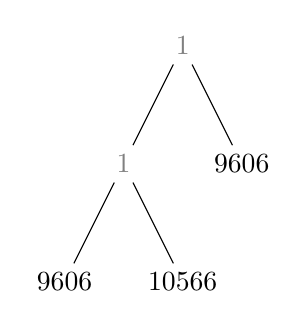
\begin{tikzpicture}
            \node [gray] {1}
            child {node [gray] {1}
            child {node {9606}}
            child {node {10566}}}
            child {node {9606}
            };
        \end{tikzpicture}
    }\hspace{0.25\textwidth}%
    \subfloat[LCA* op basis van de kinderen]{
        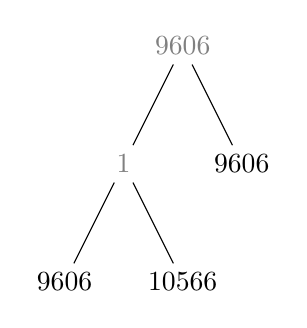
\begin{tikzpicture}
            \node [gray] {9606}
            child {node [gray] {1}
            child {node {9606}}
            child {node {10566}}}
            child {node {9606}
            };
        \end{tikzpicture}
    }
    \caption{Minimaal voorbeeld van de 2 aggregatie manieren gebruik makende van LCA*}\label{fig:lca*_diff}
\end{figure}

Onderstaande uitleg behandeld de werkwijze voor bovenstaande figuren.
\begin{itemize}
    \item Het toepassen van LCA* voor het berekenen van de top op basis van de bladeren van de boom (\{9606, 10566, 9606\}) heeft als resultaat 1 voor de root van de boom.
    9606 en 10566 zijn geen ouder of kind van elkaar, dus zal LCA* hetzelfde doen als LCA\@.
    De kleinste gemeenschappelijke ouder van deze 2 taxons is 1.
    \item Het toepassen van LCA* op basis van de directe kinderen geeft als resultaat 9606.
    Dit val simpel te verklaren aangezien de LCA* van de linker subboom 1 is.
    Als we daarna dan de LCA* van \{1, 9606\} nemen wordt 1 verwijderd aangezien dit een ouder is van 9606.
    De LCA van 9606 is natuurlijk gewoon zichzelf!
\end{itemize}

Het berekenen van de LCA* op de eerste manier is echter niet schaalbaar voor de volledige suffix boom.
Om een idee van grootorde te geven: de suffix boom voor de Swiss-Prot dataset bevat 328 922 516 toppen in het totaal, waarvan 206 523 693 bladeren.
\\ \\
Daarom hebben we uiteindelijk toch voor de standaard LCA aggregatie manier gekozen.
Deze laat wel toe de toppen op deze efficiëntere manier te aggregeren.
UMGAP biedt 2 manieren aan om LCA te doen.
Gebruik makende van RMQ (Range Minimum Queries) en een boom-gebaseerde structuur.
Zelf maak ik gebruik van de RMQ implementatie aangezien deze significant sneller was (8 min 58 sec vs 20 min en 25 sec voor de Swiss-Prot databank).
Tot slot heb ik ook eens vergeleken hoe groot de behaalde tijdswinst is bij het gebruik kunnen maken van de directe aggregatie op de kinderen, vergeleken met moeten aggregeren op de bladeren.
Bij het aggregeren op basis van de bladeren met de RMQ implementatie was de uitvoeringstijd maar liefst 12 uur, 19 minuten en 16 seconden!
Dit is dus een extreem groot verschil.

\section{Conclusie Suffix Bomen}\label{sec:conclusie-suffix-bomen}
Het is duidelijk dat suffix bomen erg performant zijn voor dit scenario.
Het opbouwen gebeurt snel en het zoeken voor een match gaat vliegensvlug.
\\ \\
Door de eigen implementatie in Rust kunnen we ook wat tijd besparen ten opzichte van een equivalente C++ implementatie.
Een deel van de winst zit tijdens het opbouwen van de boom, maar vooral tijdens het zoeken wanneer informatie uit de bladeren gehaald moet worden.
Vermoedelijk ligt de andere geheugen structuur hiervoor aan de basis.
\\ \\
Ondanks de veelbelovende resultaten op vlak van snelheid is er een keerzijde aan de medaille.
Het geheugengebruik is zo groot dat we op zoek moeten naar een andere datastructuur.
Voor de Swiss-Prot databank gaat het geheugenverbruik al boven 80 GB, terwijl ons einddoel is om dit te gebruiken op de TrEMBL dataset.
Dit wilt zeggen dat we alles \textit{slechts} $\pm$ 500 maal moeten opschalen en dan werkt het!
De oplossing is dus simpelweg een server gebruiken met ongeveer 50 TB RAM geheugen!
Of toch niet\ldots
Tijd om naar een andere datastructuur te gaan!
